% Options for packages loaded elsewhere
\PassOptionsToPackage{unicode}{hyperref}
\PassOptionsToPackage{hyphens}{url}
%
\documentclass[
]{article}
\usepackage{amsmath,amssymb}
\usepackage{lmodern}
\usepackage{iftex}
\ifPDFTeX
  \usepackage[T1]{fontenc}
  \usepackage[utf8]{inputenc}
  \usepackage{textcomp} % provide euro and other symbols
\else % if luatex or xetex
  \usepackage{unicode-math}
  \defaultfontfeatures{Scale=MatchLowercase}
  \defaultfontfeatures[\rmfamily]{Ligatures=TeX,Scale=1}
\fi
% Use upquote if available, for straight quotes in verbatim environments
\IfFileExists{upquote.sty}{\usepackage{upquote}}{}
\IfFileExists{microtype.sty}{% use microtype if available
  \usepackage[]{microtype}
  \UseMicrotypeSet[protrusion]{basicmath} % disable protrusion for tt fonts
}{}
\makeatletter
\@ifundefined{KOMAClassName}{% if non-KOMA class
  \IfFileExists{parskip.sty}{%
    \usepackage{parskip}
  }{% else
    \setlength{\parindent}{0pt}
    \setlength{\parskip}{6pt plus 2pt minus 1pt}}
}{% if KOMA class
  \KOMAoptions{parskip=half}}
\makeatother
\usepackage{xcolor}
\IfFileExists{xurl.sty}{\usepackage{xurl}}{} % add URL line breaks if available
\IfFileExists{bookmark.sty}{\usepackage{bookmark}}{\usepackage{hyperref}}
\hypersetup{
  pdftitle={BIOMAT sperimentazione},
  pdfauthor={Maurizio Giordano},
  hidelinks,
  pdfcreator={LaTeX via pandoc}}
\urlstyle{same} % disable monospaced font for URLs
\usepackage{longtable,booktabs,array}
\usepackage{calc} % for calculating minipage widths
% Correct order of tables after \paragraph or \subparagraph
\usepackage{etoolbox}
\makeatletter
\patchcmd\longtable{\par}{\if@noskipsec\mbox{}\fi\par}{}{}
\makeatother
% Allow footnotes in longtable head/foot
\IfFileExists{footnotehyper.sty}{\usepackage{footnotehyper}}{\usepackage{footnote}}
\makesavenoteenv{longtable}
\usepackage{graphicx}
\makeatletter
\def\maxwidth{\ifdim\Gin@nat@width>\linewidth\linewidth\else\Gin@nat@width\fi}
\def\maxheight{\ifdim\Gin@nat@height>\textheight\textheight\else\Gin@nat@height\fi}
\makeatother
% Scale images if necessary, so that they will not overflow the page
% margins by default, and it is still possible to overwrite the defaults
% using explicit options in \includegraphics[width, height, ...]{}
\setkeys{Gin}{width=\maxwidth,height=\maxheight,keepaspectratio}
% Set default figure placement to htbp
\makeatletter
\def\fps@figure{htbp}
\makeatother
\setlength{\emergencystretch}{3em} % prevent overfull lines
\providecommand{\tightlist}{%
  \setlength{\itemsep}{0pt}\setlength{\parskip}{0pt}}
\setcounter{secnumdepth}{-\maxdimen} % remove section numbering
\ifLuaTeX
  \usepackage{selnolig}  % disable illegal ligatures
\fi

\title{BIOMAT sperimentazione}
\author{Maurizio Giordano}
\date{10-07-2022}

\begin{document}
\maketitle

\hypertarget{label_cs_ach_most_freq-cs0-vs-cs6-9}{%
\section{label\_CS\_ACH\_most\_freq (CS0 vs
CS6-9)}\label{label_cs_ach_most_freq-cs0-vs-cs6-9}}

\hypertarget{settings}{%
\subsection{Settings}\label{settings}}

\begin{figure}
\centering
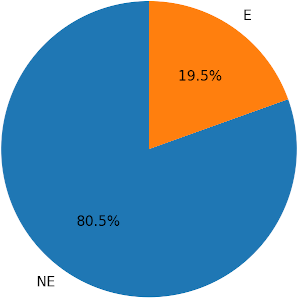
\includegraphics{figures/cs0_69.png}
\caption{CS0 vs CS6-9 distribution}
\end{figure}

\begin{itemize}
\tightlist
\item
  12538 geni complessivi - 3814 labellati
\item
  Attributi normalizzati con Z-score
\item
  5-fold cross validation
\end{itemize}

\hypertarget{ppi}{%
\subsection{PPI}\label{ppi}}

\hypertarget{biogtex}{%
\paragraph{BIO+GTEX}\label{biogtex}}

\begin{longtable}[]{@{}
  >{\raggedright\arraybackslash}p{(\columnwidth - 12\tabcolsep) * \real{0.0610}}
  >{\raggedright\arraybackslash}p{(\columnwidth - 12\tabcolsep) * \real{0.1463}}
  >{\raggedright\arraybackslash}p{(\columnwidth - 12\tabcolsep) * \real{0.1220}}
  >{\raggedright\arraybackslash}p{(\columnwidth - 12\tabcolsep) * \real{0.1829}}
  >{\raggedright\arraybackslash}p{(\columnwidth - 12\tabcolsep) * \real{0.1829}}
  >{\raggedright\arraybackslash}p{(\columnwidth - 12\tabcolsep) * \real{0.1220}}
  >{\raggedright\arraybackslash}p{(\columnwidth - 12\tabcolsep) * \real{0.1829}}@{}}
\toprule
\begin{minipage}[b]{\linewidth}\raggedright
\end{minipage} & \begin{minipage}[b]{\linewidth}\raggedright
Accuracy
\end{minipage} & \begin{minipage}[b]{\linewidth}\raggedright
BA
\end{minipage} & \begin{minipage}[b]{\linewidth}\raggedright
Sensitivity
\end{minipage} & \begin{minipage}[b]{\linewidth}\raggedright
Specificity
\end{minipage} & \begin{minipage}[b]{\linewidth}\raggedright
MCC
\end{minipage} & \begin{minipage}[b]{\linewidth}\raggedright
CM
\end{minipage} \\
\midrule
\endhead
XGB & 0.895646 & 0.806577 & 0.660403 & 0.952751 & 0.651845 & {[}{[} 492
253{]} \\
& & & & & & {[} 145 2924{]}{]} \\
MLP & 0.855275 & 0.690011 & 0.418792 & 0.961229 & 0.475601 & {[}{[} 312
433{]} \\
& & & & & & {[} 119 2950{]}{]} \\
RF & 0.879919 & 0.727178 & 0.47651 & 0.977846 & 0.574159 & {[}{[} 355
390{]} \\
& & & & & & {[} 68 3001{]}{]} \\
\bottomrule
\end{longtable}

\hypertarget{biogtexnode2vec}{%
\paragraph{BIO+GTEX+Node2Vec}\label{biogtexnode2vec}}

\begin{longtable}[]{@{}
  >{\raggedright\arraybackslash}p{(\columnwidth - 12\tabcolsep) * \real{0.0610}}
  >{\raggedright\arraybackslash}p{(\columnwidth - 12\tabcolsep) * \real{0.1463}}
  >{\raggedright\arraybackslash}p{(\columnwidth - 12\tabcolsep) * \real{0.1220}}
  >{\raggedright\arraybackslash}p{(\columnwidth - 12\tabcolsep) * \real{0.1829}}
  >{\raggedright\arraybackslash}p{(\columnwidth - 12\tabcolsep) * \real{0.1829}}
  >{\raggedright\arraybackslash}p{(\columnwidth - 12\tabcolsep) * \real{0.1220}}
  >{\raggedright\arraybackslash}p{(\columnwidth - 12\tabcolsep) * \real{0.1829}}@{}}
\toprule
\begin{minipage}[b]{\linewidth}\raggedright
\end{minipage} & \begin{minipage}[b]{\linewidth}\raggedright
Accuracy
\end{minipage} & \begin{minipage}[b]{\linewidth}\raggedright
BA
\end{minipage} & \begin{minipage}[b]{\linewidth}\raggedright
Sensitivity
\end{minipage} & \begin{minipage}[b]{\linewidth}\raggedright
Specificity
\end{minipage} & \begin{minipage}[b]{\linewidth}\raggedright
MCC
\end{minipage} & \begin{minipage}[b]{\linewidth}\raggedright
CM
\end{minipage} \\
\midrule
\endhead
XGB & 0.922654 & 0.842672 & 0.711409 & 0.973935 & \textbf{0.741349} &
{[}{[} 530 215{]} \\
& & & & & & {[} 80 2989{]}{]} \\
MLP & 0.918984 & \textbf{0.856145} & 0.75302 & 0.95927 & 0.735039 &
{[}{[} 561 184{]} \\
& & & & & & {[} 125 2944{]}{]} \\
RF & 0.899582 & 0.762774 & 0.538255 & 0.987293 & 0.652522 & {[}{[} 401
344{]} \\
& & & & & & {[} 39 3030{]}{]} \\
\bottomrule
\end{longtable}

\hypertarget{biogtexdeepwalk}{%
\paragraph{BIO+GTEX+DeepWalk}\label{biogtexdeepwalk}}

\begin{longtable}[]{@{}
  >{\raggedright\arraybackslash}p{(\columnwidth - 12\tabcolsep) * \real{0.0610}}
  >{\raggedright\arraybackslash}p{(\columnwidth - 12\tabcolsep) * \real{0.1463}}
  >{\raggedright\arraybackslash}p{(\columnwidth - 12\tabcolsep) * \real{0.1220}}
  >{\raggedright\arraybackslash}p{(\columnwidth - 12\tabcolsep) * \real{0.1829}}
  >{\raggedright\arraybackslash}p{(\columnwidth - 12\tabcolsep) * \real{0.1829}}
  >{\raggedright\arraybackslash}p{(\columnwidth - 12\tabcolsep) * \real{0.1220}}
  >{\raggedright\arraybackslash}p{(\columnwidth - 12\tabcolsep) * \real{0.1829}}@{}}
\toprule
\begin{minipage}[b]{\linewidth}\raggedright
\end{minipage} & \begin{minipage}[b]{\linewidth}\raggedright
Accuracy
\end{minipage} & \begin{minipage}[b]{\linewidth}\raggedright
BA
\end{minipage} & \begin{minipage}[b]{\linewidth}\raggedright
Sensitivity
\end{minipage} & \begin{minipage}[b]{\linewidth}\raggedright
Specificity
\end{minipage} & \begin{minipage}[b]{\linewidth}\raggedright
MCC
\end{minipage} & \begin{minipage}[b]{\linewidth}\raggedright
CM
\end{minipage} \\
\midrule
\endhead
XGB & 0.923177 & 0.839947 & 0.703356 & 0.976538 & \textbf{0.742353} &
{[}{[} 524 221{]} \\
& & & & & & {[} 72 2997{]}{]} \\
MLP & 0.917932 & \textbf{0.851427} & 0.742282 & 0.960571 & 0.730933 &
{[}{[} 553 192{]} \\
& & & & & & {[} 121 2948{]}{]} \\
RF & 0.896962 & 0.755046 & 0.522148 & 0.987944 & 0.641838 & {[}{[} 389
356{]} \\
& & & & & & {[} 37 3032{]}{]} \\
\bottomrule
\end{longtable}

\hypertarget{biogtexhope}{%
\paragraph{BIO+GTEX+HOPE}\label{biogtexhope}}

\begin{longtable}[]{@{}
  >{\raggedright\arraybackslash}p{(\columnwidth - 12\tabcolsep) * \real{0.0625}}
  >{\raggedright\arraybackslash}p{(\columnwidth - 12\tabcolsep) * \real{0.1500}}
  >{\raggedright\arraybackslash}p{(\columnwidth - 12\tabcolsep) * \real{0.1125}}
  >{\raggedright\arraybackslash}p{(\columnwidth - 12\tabcolsep) * \real{0.1875}}
  >{\raggedright\arraybackslash}p{(\columnwidth - 12\tabcolsep) * \real{0.1875}}
  >{\raggedright\arraybackslash}p{(\columnwidth - 12\tabcolsep) * \real{0.1125}}
  >{\raggedright\arraybackslash}p{(\columnwidth - 12\tabcolsep) * \real{0.1875}}@{}}
\toprule
\begin{minipage}[b]{\linewidth}\raggedright
\end{minipage} & \begin{minipage}[b]{\linewidth}\raggedright
Accuracy
\end{minipage} & \begin{minipage}[b]{\linewidth}\raggedright
BA
\end{minipage} & \begin{minipage}[b]{\linewidth}\raggedright
Sensitivity
\end{minipage} & \begin{minipage}[b]{\linewidth}\raggedright
Specificity
\end{minipage} & \begin{minipage}[b]{\linewidth}\raggedright
MCC
\end{minipage} & \begin{minipage}[b]{\linewidth}\raggedright
CM
\end{minipage} \\
\midrule
\endhead
XGB & 0.904826 & 0.81838 & 0.67651 & 0.96025 & 0.68186 & {[}{[} 504
241{]} \\
& & & & & & {[} 122 2947{]}{]} \\
MLP & 0.850291 & 0.740279 & 0.559732 & 0.920827 & 0.504984 & {[}{[} 417
328{]} \\
& & & & & & {[} 243 2826{]}{]} \\
RF & 0.869166 & 0.721006 & 0.477852 & 0.96416 & 0.535904 & {[}{[} 356
389{]} \\
& & & & & & {[} 110 2959{]}{]} \\
\bottomrule
\end{longtable}

\hypertarget{met}{%
\subsection{MET}\label{met}}

\hypertarget{biogtex-1}{%
\paragraph{BIO+GTEX}\label{biogtex-1}}

\begin{longtable}[]{@{}
  >{\raggedright\arraybackslash}p{(\columnwidth - 12\tabcolsep) * \real{0.0625}}
  >{\raggedright\arraybackslash}p{(\columnwidth - 12\tabcolsep) * \real{0.1500}}
  >{\raggedright\arraybackslash}p{(\columnwidth - 12\tabcolsep) * \real{0.1250}}
  >{\raggedright\arraybackslash}p{(\columnwidth - 12\tabcolsep) * \real{0.1875}}
  >{\raggedright\arraybackslash}p{(\columnwidth - 12\tabcolsep) * \real{0.1875}}
  >{\raggedright\arraybackslash}p{(\columnwidth - 12\tabcolsep) * \real{0.1000}}
  >{\raggedright\arraybackslash}p{(\columnwidth - 12\tabcolsep) * \real{0.1875}}@{}}
\toprule
\begin{minipage}[b]{\linewidth}\raggedright
\end{minipage} & \begin{minipage}[b]{\linewidth}\raggedright
Accuracy
\end{minipage} & \begin{minipage}[b]{\linewidth}\raggedright
BA
\end{minipage} & \begin{minipage}[b]{\linewidth}\raggedright
Sensitivity
\end{minipage} & \begin{minipage}[b]{\linewidth}\raggedright
Specificity
\end{minipage} & \begin{minipage}[b]{\linewidth}\raggedright
MCC
\end{minipage} & \begin{minipage}[b]{\linewidth}\raggedright
CM
\end{minipage} \\
\midrule
\endhead
XGB & 0.898268 & 0.813797 & 0.675168 & 0.952425 & 0.662255 & {[}{[} 503
242{]} \\
& & & & & & {[} 146 2923{]}{]} \\
MLP & 0.851865 & 0.682809 & 0.405369 & 0.960249 & 0.459727 & {[}{[} 302
443{]} \\
& & & & & & {[} 122 2947{]}{]} \\
\bottomrule
\end{longtable}

\hypertarget{biogtexnode2vec-1}{%
\paragraph{BIO+GTEX+Node2Vec}\label{biogtexnode2vec-1}}

\begin{longtable}[]{@{}
  >{\raggedright\arraybackslash}p{(\columnwidth - 12\tabcolsep) * \real{0.0610}}
  >{\raggedright\arraybackslash}p{(\columnwidth - 12\tabcolsep) * \real{0.1463}}
  >{\raggedright\arraybackslash}p{(\columnwidth - 12\tabcolsep) * \real{0.1220}}
  >{\raggedright\arraybackslash}p{(\columnwidth - 12\tabcolsep) * \real{0.1829}}
  >{\raggedright\arraybackslash}p{(\columnwidth - 12\tabcolsep) * \real{0.1829}}
  >{\raggedright\arraybackslash}p{(\columnwidth - 12\tabcolsep) * \real{0.1220}}
  >{\raggedright\arraybackslash}p{(\columnwidth - 12\tabcolsep) * \real{0.1829}}@{}}
\toprule
\begin{minipage}[b]{\linewidth}\raggedright
\end{minipage} & \begin{minipage}[b]{\linewidth}\raggedright
Accuracy
\end{minipage} & \begin{minipage}[b]{\linewidth}\raggedright
BA
\end{minipage} & \begin{minipage}[b]{\linewidth}\raggedright
Sensitivity
\end{minipage} & \begin{minipage}[b]{\linewidth}\raggedright
Specificity
\end{minipage} & \begin{minipage}[b]{\linewidth}\raggedright
MCC
\end{minipage} & \begin{minipage}[b]{\linewidth}\raggedright
CM
\end{minipage} \\
\midrule
\endhead
XGB & 0.888308 & 0.780163 & 0.602685 & 0.957642 & 0.619234 & {[}{[} 449
296{]} \\
& & & & & & {[} 130 2939{]}{]} \\
MLP & 0.812011 & 0.656522 & 0.401342 & 0.911701 & 0.348635 & {[}{[} 299
446{]} \\
& & & & & & {[} 271 2798{]}{]} \\
\bottomrule
\end{longtable}

\hypertarget{biogtexdeepwalk-1}{%
\paragraph{BIO+GTEX+DeepWalk}\label{biogtexdeepwalk-1}}

\begin{longtable}[]{@{}
  >{\raggedright\arraybackslash}p{(\columnwidth - 12\tabcolsep) * \real{0.0610}}
  >{\raggedright\arraybackslash}p{(\columnwidth - 12\tabcolsep) * \real{0.1463}}
  >{\raggedright\arraybackslash}p{(\columnwidth - 12\tabcolsep) * \real{0.1220}}
  >{\raggedright\arraybackslash}p{(\columnwidth - 12\tabcolsep) * \real{0.1829}}
  >{\raggedright\arraybackslash}p{(\columnwidth - 12\tabcolsep) * \real{0.1829}}
  >{\raggedright\arraybackslash}p{(\columnwidth - 12\tabcolsep) * \real{0.1220}}
  >{\raggedright\arraybackslash}p{(\columnwidth - 12\tabcolsep) * \real{0.1829}}@{}}
\toprule
\begin{minipage}[b]{\linewidth}\raggedright
\end{minipage} & \begin{minipage}[b]{\linewidth}\raggedright
Accuracy
\end{minipage} & \begin{minipage}[b]{\linewidth}\raggedright
BA
\end{minipage} & \begin{minipage}[b]{\linewidth}\raggedright
Sensitivity
\end{minipage} & \begin{minipage}[b]{\linewidth}\raggedright
Specificity
\end{minipage} & \begin{minipage}[b]{\linewidth}\raggedright
MCC
\end{minipage} & \begin{minipage}[b]{\linewidth}\raggedright
CM
\end{minipage} \\
\midrule
\endhead
XGB & 0.886733 & 0.776644 & 0.595973 & 0.957315 & 0.613232 & {[}{[} 444
301{]} \\
& & & & & & {[} 131 2938{]}{]} \\
MLP & 0.817516 & 0.665533 & 0.416107 & 0.914958 & 0.36788 & {[}{[} 310
435{]} \\
& & & & & & {[} 261 2808{]}{]} \\
\bottomrule
\end{longtable}

\hypertarget{biogtexhope-1}{%
\paragraph{BIO+GTEX+HOPE}\label{biogtexhope-1}}

\begin{longtable}[]{@{}
  >{\raggedright\arraybackslash}p{(\columnwidth - 12\tabcolsep) * \real{0.0610}}
  >{\raggedright\arraybackslash}p{(\columnwidth - 12\tabcolsep) * \real{0.1463}}
  >{\raggedright\arraybackslash}p{(\columnwidth - 12\tabcolsep) * \real{0.1220}}
  >{\raggedright\arraybackslash}p{(\columnwidth - 12\tabcolsep) * \real{0.1829}}
  >{\raggedright\arraybackslash}p{(\columnwidth - 12\tabcolsep) * \real{0.1829}}
  >{\raggedright\arraybackslash}p{(\columnwidth - 12\tabcolsep) * \real{0.1220}}
  >{\raggedright\arraybackslash}p{(\columnwidth - 12\tabcolsep) * \real{0.1829}}@{}}
\toprule
\begin{minipage}[b]{\linewidth}\raggedright
\end{minipage} & \begin{minipage}[b]{\linewidth}\raggedright
Accuracy
\end{minipage} & \begin{minipage}[b]{\linewidth}\raggedright
BA
\end{minipage} & \begin{minipage}[b]{\linewidth}\raggedright
Sensitivity
\end{minipage} & \begin{minipage}[b]{\linewidth}\raggedright
Specificity
\end{minipage} & \begin{minipage}[b]{\linewidth}\raggedright
MCC
\end{minipage} & \begin{minipage}[b]{\linewidth}\raggedright
CM
\end{minipage} \\
\midrule
\endhead
XGB & 0.89643 & 0.810114 & 0.668456 & 0.951771 & 0.656043 & {[}{[} 498
247{]} \\
& & & & & & {[} 148 2921{]}{]} \\
MLP & 0.821444 & 0.629857 & 0.315436 & 0.944277 & 0.335774 & {[}{[} 235
510{]} \\
& & & & & & {[} 171 2898{]}{]} \\
\bottomrule
\end{longtable}

\hypertarget{metppi}{%
\subsection{MET+PPI}\label{metppi}}

\hypertarget{biogtex-2}{%
\paragraph{BIO+GTEX}\label{biogtex-2}}

\begin{longtable}[]{@{}
  >{\raggedright\arraybackslash}p{(\columnwidth - 12\tabcolsep) * \real{0.0610}}
  >{\raggedright\arraybackslash}p{(\columnwidth - 12\tabcolsep) * \real{0.1463}}
  >{\raggedright\arraybackslash}p{(\columnwidth - 12\tabcolsep) * \real{0.1220}}
  >{\raggedright\arraybackslash}p{(\columnwidth - 12\tabcolsep) * \real{0.1829}}
  >{\raggedright\arraybackslash}p{(\columnwidth - 12\tabcolsep) * \real{0.1829}}
  >{\raggedright\arraybackslash}p{(\columnwidth - 12\tabcolsep) * \real{0.1220}}
  >{\raggedright\arraybackslash}p{(\columnwidth - 12\tabcolsep) * \real{0.1829}}@{}}
\toprule
\begin{minipage}[b]{\linewidth}\raggedright
\end{minipage} & \begin{minipage}[b]{\linewidth}\raggedright
Accuracy
\end{minipage} & \begin{minipage}[b]{\linewidth}\raggedright
BA
\end{minipage} & \begin{minipage}[b]{\linewidth}\raggedright
Sensitivity
\end{minipage} & \begin{minipage}[b]{\linewidth}\raggedright
Specificity
\end{minipage} & \begin{minipage}[b]{\linewidth}\raggedright
MCC
\end{minipage} & \begin{minipage}[b]{\linewidth}\raggedright
CM
\end{minipage} \\
\midrule
\endhead
XGB & 0.898531 & 0.809385 & 0.663087 & 0.955682 & 0.660859 & {[}{[} 494
251{]} \\
& & & & & & {[} 136 2933{]}{]} \\
MLP & 0.85606 & 0.68999 & 0.41745 & 0.962531 & 0.477454 & {[}{[} 311
434{]} \\
& & & & & & {[} 115 2954{]}{]} \\
\bottomrule
\end{longtable}

\hypertarget{biogtexnode2vec-2}{%
\paragraph{BIO+GTEX+Node2Vec}\label{biogtexnode2vec-2}}

\begin{longtable}[]{@{}
  >{\raggedright\arraybackslash}p{(\columnwidth - 12\tabcolsep) * \real{0.0610}}
  >{\raggedright\arraybackslash}p{(\columnwidth - 12\tabcolsep) * \real{0.1463}}
  >{\raggedright\arraybackslash}p{(\columnwidth - 12\tabcolsep) * \real{0.1220}}
  >{\raggedright\arraybackslash}p{(\columnwidth - 12\tabcolsep) * \real{0.1829}}
  >{\raggedright\arraybackslash}p{(\columnwidth - 12\tabcolsep) * \real{0.1829}}
  >{\raggedright\arraybackslash}p{(\columnwidth - 12\tabcolsep) * \real{0.1220}}
  >{\raggedright\arraybackslash}p{(\columnwidth - 12\tabcolsep) * \real{0.1829}}@{}}
\toprule
\begin{minipage}[b]{\linewidth}\raggedright
\end{minipage} & \begin{minipage}[b]{\linewidth}\raggedright
Accuracy
\end{minipage} & \begin{minipage}[b]{\linewidth}\raggedright
BA
\end{minipage} & \begin{minipage}[b]{\linewidth}\raggedright
Sensitivity
\end{minipage} & \begin{minipage}[b]{\linewidth}\raggedright
Specificity
\end{minipage} & \begin{minipage}[b]{\linewidth}\raggedright
MCC
\end{minipage} & \begin{minipage}[b]{\linewidth}\raggedright
CM
\end{minipage} \\
\midrule
\endhead
XGB & 0.923966 & 0.849077 & 0.726174 & 0.97198 & \textbf{0.746896} &
{[}{[} 541 204{]} \\
& & & & & & {[} 86 2983{]}{]} \\
MLP & 0.912691 & 0.844103 & 0.731544 & 0.956662 & 0.713719 & {[}{[} 545
200{]} \\
& & & & & & {[} 133 2936{]}{]} \\
\bottomrule
\end{longtable}

\hypertarget{biogtexdeepwalk-2}{%
\paragraph{BIO+GTEX+DeepWalk}\label{biogtexdeepwalk-2}}

\begin{longtable}[]{@{}
  >{\raggedright\arraybackslash}p{(\columnwidth - 12\tabcolsep) * \real{0.0617}}
  >{\raggedright\arraybackslash}p{(\columnwidth - 12\tabcolsep) * \real{0.1481}}
  >{\raggedright\arraybackslash}p{(\columnwidth - 12\tabcolsep) * \real{0.1235}}
  >{\raggedright\arraybackslash}p{(\columnwidth - 12\tabcolsep) * \real{0.1852}}
  >{\raggedright\arraybackslash}p{(\columnwidth - 12\tabcolsep) * \real{0.1852}}
  >{\raggedright\arraybackslash}p{(\columnwidth - 12\tabcolsep) * \real{0.1111}}
  >{\raggedright\arraybackslash}p{(\columnwidth - 12\tabcolsep) * \real{0.1852}}@{}}
\toprule
\begin{minipage}[b]{\linewidth}\raggedright
\end{minipage} & \begin{minipage}[b]{\linewidth}\raggedright
Accuracy
\end{minipage} & \begin{minipage}[b]{\linewidth}\raggedright
BA
\end{minipage} & \begin{minipage}[b]{\linewidth}\raggedright
Sensitivity
\end{minipage} & \begin{minipage}[b]{\linewidth}\raggedright
Specificity
\end{minipage} & \begin{minipage}[b]{\linewidth}\raggedright
MCC
\end{minipage} & \begin{minipage}[b]{\linewidth}\raggedright
CM
\end{minipage} \\
\midrule
\endhead
XGB & 0.921606 & 0.842528 & 0.712752 & 0.972305 & \textbf{0.73816} &
{[}{[} 531 214{]} \\
& & & & & & {[} 85 2984{]}{]} \\
MLP & 0.918719 & 0.855981 & 0.75302 & 0.958942 & 0.735141 & {[}{[} 561
184{]} \\
& & & & & & {[} 126 2943{]}{]} \\
\bottomrule
\end{longtable}

\hypertarget{biogtexhope-2}{%
\paragraph{BIO+GTEX+HOPE}\label{biogtexhope-2}}

\begin{longtable}[]{@{}
  >{\raggedright\arraybackslash}p{(\columnwidth - 12\tabcolsep) * \real{0.0610}}
  >{\raggedright\arraybackslash}p{(\columnwidth - 12\tabcolsep) * \real{0.1463}}
  >{\raggedright\arraybackslash}p{(\columnwidth - 12\tabcolsep) * \real{0.1220}}
  >{\raggedright\arraybackslash}p{(\columnwidth - 12\tabcolsep) * \real{0.1829}}
  >{\raggedright\arraybackslash}p{(\columnwidth - 12\tabcolsep) * \real{0.1829}}
  >{\raggedright\arraybackslash}p{(\columnwidth - 12\tabcolsep) * \real{0.1220}}
  >{\raggedright\arraybackslash}p{(\columnwidth - 12\tabcolsep) * \real{0.1829}}@{}}
\toprule
\begin{minipage}[b]{\linewidth}\raggedright
\end{minipage} & \begin{minipage}[b]{\linewidth}\raggedright
Accuracy
\end{minipage} & \begin{minipage}[b]{\linewidth}\raggedright
BA
\end{minipage} & \begin{minipage}[b]{\linewidth}\raggedright
Sensitivity
\end{minipage} & \begin{minipage}[b]{\linewidth}\raggedright
Specificity
\end{minipage} & \begin{minipage}[b]{\linewidth}\raggedright
MCC
\end{minipage} & \begin{minipage}[b]{\linewidth}\raggedright
CM
\end{minipage} \\
\midrule
\endhead
XGB & 0.901151 & 0.813047 & 0.668456 & 0.957638 & 0.669963 & {[}{[} 498
247{]} \\
& & & & & & {[} 130 2939{]}{]} \\
MLP & 0.806504 & 0.688677 & 0.495302 & 0.882053 & 0.38051 & {[}{[} 369
376{]} \\
& & & & & & {[} 362 2707{]}{]} \\
\bottomrule
\end{longtable}

\hypertarget{label_cs_ach_most_freq-cs0-1-vs-cs6-9}{%
\section{label\_CS\_ACH\_most\_freq (CS0-1 vs
CS6-9)}\label{label_cs_ach_most_freq-cs0-1-vs-cs6-9}}

\hypertarget{settings-1}{%
\subsection{Settings}\label{settings-1}}

\begin{figure}
\centering
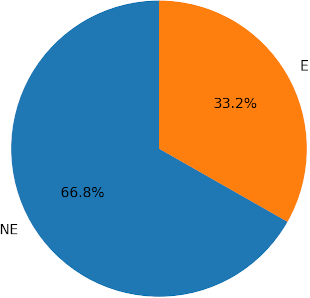
\includegraphics{figures/cs01_69.png}
\caption{CS0-1 vs CS6-9 distribution}
\end{figure}

\begin{itemize}
\tightlist
\item
  12538 geni complessivi - 4596 labellati
\item
  Attributi normalizzati con Z-score
\item
  5-fold cross validation
\end{itemize}

\hypertarget{ppi-1}{%
\subsection{PPI}\label{ppi-1}}

\hypertarget{biogtex-3}{%
\paragraph{BIO+GTEX}\label{biogtex-3}}

\begin{longtable}[]{@{}
  >{\raggedright\arraybackslash}p{(\columnwidth - 12\tabcolsep) * \real{0.0610}}
  >{\raggedright\arraybackslash}p{(\columnwidth - 12\tabcolsep) * \real{0.1463}}
  >{\raggedright\arraybackslash}p{(\columnwidth - 12\tabcolsep) * \real{0.1220}}
  >{\raggedright\arraybackslash}p{(\columnwidth - 12\tabcolsep) * \real{0.1829}}
  >{\raggedright\arraybackslash}p{(\columnwidth - 12\tabcolsep) * \real{0.1829}}
  >{\raggedright\arraybackslash}p{(\columnwidth - 12\tabcolsep) * \real{0.1220}}
  >{\raggedright\arraybackslash}p{(\columnwidth - 12\tabcolsep) * \real{0.1829}}@{}}
\toprule
\begin{minipage}[b]{\linewidth}\raggedright
\end{minipage} & \begin{minipage}[b]{\linewidth}\raggedright
Accuracy
\end{minipage} & \begin{minipage}[b]{\linewidth}\raggedright
BA
\end{minipage} & \begin{minipage}[b]{\linewidth}\raggedright
Sensitivity
\end{minipage} & \begin{minipage}[b]{\linewidth}\raggedright
Specificity
\end{minipage} & \begin{minipage}[b]{\linewidth}\raggedright
MCC
\end{minipage} & \begin{minipage}[b]{\linewidth}\raggedright
CM
\end{minipage} \\
\midrule
\endhead
XGB & 0.834859 & 0.805927 & 0.719706 & 0.892147 & 0.622746 & {[}{[}1099
428{]} \\
& & & & & & {[} 331 2738{]}{]} \\
\bottomrule
\end{longtable}

\hypertarget{biogtexnode2vec-3}{%
\paragraph{BIO+GTEX+Node2Vec}\label{biogtexnode2vec-3}}

\begin{longtable}[]{@{}
  >{\raggedright\arraybackslash}p{(\columnwidth - 12\tabcolsep) * \real{0.0610}}
  >{\raggedright\arraybackslash}p{(\columnwidth - 12\tabcolsep) * \real{0.1463}}
  >{\raggedright\arraybackslash}p{(\columnwidth - 12\tabcolsep) * \real{0.1220}}
  >{\raggedright\arraybackslash}p{(\columnwidth - 12\tabcolsep) * \real{0.1829}}
  >{\raggedright\arraybackslash}p{(\columnwidth - 12\tabcolsep) * \real{0.1829}}
  >{\raggedright\arraybackslash}p{(\columnwidth - 12\tabcolsep) * \real{0.1220}}
  >{\raggedright\arraybackslash}p{(\columnwidth - 12\tabcolsep) * \real{0.1829}}@{}}
\toprule
\begin{minipage}[b]{\linewidth}\raggedright
\end{minipage} & \begin{minipage}[b]{\linewidth}\raggedright
Accuracy
\end{minipage} & \begin{minipage}[b]{\linewidth}\raggedright
BA
\end{minipage} & \begin{minipage}[b]{\linewidth}\raggedright
Sensitivity
\end{minipage} & \begin{minipage}[b]{\linewidth}\raggedright
Specificity
\end{minipage} & \begin{minipage}[b]{\linewidth}\raggedright
MCC
\end{minipage} & \begin{minipage}[b]{\linewidth}\raggedright
CM
\end{minipage} \\
\midrule
\endhead
XGB & 0.87141 & 0.843989 & 0.762265 & 0.925713 & \textbf{0.705343} &
{[}{[}1164 363{]} \\
& & & & & & {[} 228 2841{]}{]} \\
\bottomrule
\end{longtable}

\hypertarget{biogtexdeepwalk-3}{%
\paragraph{BIO+GTEX+DeepWalk}\label{biogtexdeepwalk-3}}

\begin{longtable}[]{@{}
  >{\raggedright\arraybackslash}p{(\columnwidth - 12\tabcolsep) * \real{0.0610}}
  >{\raggedright\arraybackslash}p{(\columnwidth - 12\tabcolsep) * \real{0.1463}}
  >{\raggedright\arraybackslash}p{(\columnwidth - 12\tabcolsep) * \real{0.1220}}
  >{\raggedright\arraybackslash}p{(\columnwidth - 12\tabcolsep) * \real{0.1829}}
  >{\raggedright\arraybackslash}p{(\columnwidth - 12\tabcolsep) * \real{0.1829}}
  >{\raggedright\arraybackslash}p{(\columnwidth - 12\tabcolsep) * \real{0.1220}}
  >{\raggedright\arraybackslash}p{(\columnwidth - 12\tabcolsep) * \real{0.1829}}@{}}
\toprule
\begin{minipage}[b]{\linewidth}\raggedright
\end{minipage} & \begin{minipage}[b]{\linewidth}\raggedright
Accuracy
\end{minipage} & \begin{minipage}[b]{\linewidth}\raggedright
BA
\end{minipage} & \begin{minipage}[b]{\linewidth}\raggedright
Sensitivity
\end{minipage} & \begin{minipage}[b]{\linewidth}\raggedright
Specificity
\end{minipage} & \begin{minipage}[b]{\linewidth}\raggedright
MCC
\end{minipage} & \begin{minipage}[b]{\linewidth}\raggedright
CM
\end{minipage} \\
\midrule
\endhead
XGB & 0.86619 & 0.838436 & 0.755725 & 0.921147 & 0.693355 & {[}{[}1154
373{]} \\
& & & & & & {[} 242 2827{]}{]} \\
\bottomrule
\end{longtable}

\hypertarget{biogtexhope-3}{%
\paragraph{BIO+GTEX+HOPE}\label{biogtexhope-3}}

\begin{longtable}[]{@{}
  >{\raggedright\arraybackslash}p{(\columnwidth - 12\tabcolsep) * \real{0.0625}}
  >{\raggedright\arraybackslash}p{(\columnwidth - 12\tabcolsep) * \real{0.1500}}
  >{\raggedright\arraybackslash}p{(\columnwidth - 12\tabcolsep) * \real{0.1125}}
  >{\raggedright\arraybackslash}p{(\columnwidth - 12\tabcolsep) * \real{0.1875}}
  >{\raggedright\arraybackslash}p{(\columnwidth - 12\tabcolsep) * \real{0.1875}}
  >{\raggedright\arraybackslash}p{(\columnwidth - 12\tabcolsep) * \real{0.1125}}
  >{\raggedright\arraybackslash}p{(\columnwidth - 12\tabcolsep) * \real{0.1875}}@{}}
\toprule
\begin{minipage}[b]{\linewidth}\raggedright
\end{minipage} & \begin{minipage}[b]{\linewidth}\raggedright
Accuracy
\end{minipage} & \begin{minipage}[b]{\linewidth}\raggedright
BA
\end{minipage} & \begin{minipage}[b]{\linewidth}\raggedright
Sensitivity
\end{minipage} & \begin{minipage}[b]{\linewidth}\raggedright
Specificity
\end{minipage} & \begin{minipage}[b]{\linewidth}\raggedright
MCC
\end{minipage} & \begin{minipage}[b]{\linewidth}\raggedright
CM
\end{minipage} \\
\midrule
\endhead
XGB & 0.844431 & 0.814736 & 0.726242 & 0.90323 & 0.643618 & {[}{[}1109
418{]} \\
& & & & & & {[} 297 2772{]}{]} \\
\bottomrule
\end{longtable}

\hypertarget{met-1}{%
\subsection{MET}\label{met-1}}

\hypertarget{biogtex-4}{%
\paragraph{BIO+GTEX}\label{biogtex-4}}

\begin{longtable}[]{@{}
  >{\raggedright\arraybackslash}p{(\columnwidth - 12\tabcolsep) * \real{0.0625}}
  >{\raggedright\arraybackslash}p{(\columnwidth - 12\tabcolsep) * \real{0.1500}}
  >{\raggedright\arraybackslash}p{(\columnwidth - 12\tabcolsep) * \real{0.1250}}
  >{\raggedright\arraybackslash}p{(\columnwidth - 12\tabcolsep) * \real{0.1875}}
  >{\raggedright\arraybackslash}p{(\columnwidth - 12\tabcolsep) * \real{0.1875}}
  >{\raggedright\arraybackslash}p{(\columnwidth - 12\tabcolsep) * \real{0.1000}}
  >{\raggedright\arraybackslash}p{(\columnwidth - 12\tabcolsep) * \real{0.1875}}@{}}
\toprule
\begin{minipage}[b]{\linewidth}\raggedright
\end{minipage} & \begin{minipage}[b]{\linewidth}\raggedright
Accuracy
\end{minipage} & \begin{minipage}[b]{\linewidth}\raggedright
BA
\end{minipage} & \begin{minipage}[b]{\linewidth}\raggedright
Sensitivity
\end{minipage} & \begin{minipage}[b]{\linewidth}\raggedright
Specificity
\end{minipage} & \begin{minipage}[b]{\linewidth}\raggedright
MCC
\end{minipage} & \begin{minipage}[b]{\linewidth}\raggedright
CM
\end{minipage} \\
\midrule
\endhead
XGB & 0.835512 & 0.808063 & 0.72626 & 0.889866 & 0.624804 & {[}{[}1109
418{]} \\
& & & & & & {[} 338 2731{]}{]} \\
\bottomrule
\end{longtable}

\hypertarget{biogtexnode2vec-4}{%
\paragraph{BIO+GTEX+Node2Vec}\label{biogtexnode2vec-4}}

\begin{longtable}[]{@{}
  >{\raggedright\arraybackslash}p{(\columnwidth - 12\tabcolsep) * \real{0.0610}}
  >{\raggedright\arraybackslash}p{(\columnwidth - 12\tabcolsep) * \real{0.1463}}
  >{\raggedright\arraybackslash}p{(\columnwidth - 12\tabcolsep) * \real{0.1220}}
  >{\raggedright\arraybackslash}p{(\columnwidth - 12\tabcolsep) * \real{0.1829}}
  >{\raggedright\arraybackslash}p{(\columnwidth - 12\tabcolsep) * \real{0.1829}}
  >{\raggedright\arraybackslash}p{(\columnwidth - 12\tabcolsep) * \real{0.1220}}
  >{\raggedright\arraybackslash}p{(\columnwidth - 12\tabcolsep) * \real{0.1829}}@{}}
\toprule
\begin{minipage}[b]{\linewidth}\raggedright
\end{minipage} & \begin{minipage}[b]{\linewidth}\raggedright
Accuracy
\end{minipage} & \begin{minipage}[b]{\linewidth}\raggedright
BA
\end{minipage} & \begin{minipage}[b]{\linewidth}\raggedright
Sensitivity
\end{minipage} & \begin{minipage}[b]{\linewidth}\raggedright
Specificity
\end{minipage} & \begin{minipage}[b]{\linewidth}\raggedright
MCC
\end{minipage} & \begin{minipage}[b]{\linewidth}\raggedright
CM
\end{minipage} \\
\midrule
\endhead
XGB & 0.81941 & 0.784651 & 0.681067 & 0.888235 & 0.584655 & {[}{[}1040
487{]} \\
& & & & & & {[} 343 2726{]}{]} \\
\bottomrule
\end{longtable}

\hypertarget{biogtexdeepwalk-4}{%
\paragraph{BIO+GTEX+DeepWalk}\label{biogtexdeepwalk-4}}

\begin{longtable}[]{@{}
  >{\raggedright\arraybackslash}p{(\columnwidth - 12\tabcolsep) * \real{0.0610}}
  >{\raggedright\arraybackslash}p{(\columnwidth - 12\tabcolsep) * \real{0.1463}}
  >{\raggedright\arraybackslash}p{(\columnwidth - 12\tabcolsep) * \real{0.1220}}
  >{\raggedright\arraybackslash}p{(\columnwidth - 12\tabcolsep) * \real{0.1829}}
  >{\raggedright\arraybackslash}p{(\columnwidth - 12\tabcolsep) * \real{0.1829}}
  >{\raggedright\arraybackslash}p{(\columnwidth - 12\tabcolsep) * \real{0.1220}}
  >{\raggedright\arraybackslash}p{(\columnwidth - 12\tabcolsep) * \real{0.1829}}@{}}
\toprule
\begin{minipage}[b]{\linewidth}\raggedright
\end{minipage} & \begin{minipage}[b]{\linewidth}\raggedright
Accuracy
\end{minipage} & \begin{minipage}[b]{\linewidth}\raggedright
BA
\end{minipage} & \begin{minipage}[b]{\linewidth}\raggedright
Sensitivity
\end{minipage} & \begin{minipage}[b]{\linewidth}\raggedright
Specificity
\end{minipage} & \begin{minipage}[b]{\linewidth}\raggedright
MCC
\end{minipage} & \begin{minipage}[b]{\linewidth}\raggedright
CM
\end{minipage} \\
\midrule
\endhead
XGB & 0.823112 & 0.790231 & 0.692228 & 0.888235 & 0.59403 & {[}{[}1057
470{]} \\
& & & & & & {[} 343 2726{]}{]} \\
\bottomrule
\end{longtable}

\hypertarget{biogtexhope-4}{%
\paragraph{BIO+GTEX+HOPE}\label{biogtexhope-4}}

\begin{longtable}[]{@{}
  >{\raggedright\arraybackslash}p{(\columnwidth - 12\tabcolsep) * \real{0.0610}}
  >{\raggedright\arraybackslash}p{(\columnwidth - 12\tabcolsep) * \real{0.1463}}
  >{\raggedright\arraybackslash}p{(\columnwidth - 12\tabcolsep) * \real{0.1220}}
  >{\raggedright\arraybackslash}p{(\columnwidth - 12\tabcolsep) * \real{0.1829}}
  >{\raggedright\arraybackslash}p{(\columnwidth - 12\tabcolsep) * \real{0.1829}}
  >{\raggedright\arraybackslash}p{(\columnwidth - 12\tabcolsep) * \real{0.1220}}
  >{\raggedright\arraybackslash}p{(\columnwidth - 12\tabcolsep) * \real{0.1829}}@{}}
\toprule
\begin{minipage}[b]{\linewidth}\raggedright
\end{minipage} & \begin{minipage}[b]{\linewidth}\raggedright
Accuracy
\end{minipage} & \begin{minipage}[b]{\linewidth}\raggedright
BA
\end{minipage} & \begin{minipage}[b]{\linewidth}\raggedright
Sensitivity
\end{minipage} & \begin{minipage}[b]{\linewidth}\raggedright
Specificity
\end{minipage} & \begin{minipage}[b]{\linewidth}\raggedright
MCC
\end{minipage} & \begin{minipage}[b]{\linewidth}\raggedright
CM
\end{minipage} \\
\midrule
\endhead
XGB & 0.838556 & 0.810175 & 0.725597 & 0.894753 & 0.631054 & {[}{[}1108
419{]} \\
& & & & & & {[} 323 2746{]}{]} \\
\bottomrule
\end{longtable}

\hypertarget{metppi-1}{%
\subsection{MET+PPI}\label{metppi-1}}

\hypertarget{biogtex-5}{%
\paragraph{BIO+GTEX}\label{biogtex-5}}

\begin{longtable}[]{@{}
  >{\raggedright\arraybackslash}p{(\columnwidth - 12\tabcolsep) * \real{0.0610}}
  >{\raggedright\arraybackslash}p{(\columnwidth - 12\tabcolsep) * \real{0.1463}}
  >{\raggedright\arraybackslash}p{(\columnwidth - 12\tabcolsep) * \real{0.1220}}
  >{\raggedright\arraybackslash}p{(\columnwidth - 12\tabcolsep) * \real{0.1829}}
  >{\raggedright\arraybackslash}p{(\columnwidth - 12\tabcolsep) * \real{0.1829}}
  >{\raggedright\arraybackslash}p{(\columnwidth - 12\tabcolsep) * \real{0.1220}}
  >{\raggedright\arraybackslash}p{(\columnwidth - 12\tabcolsep) * \real{0.1829}}@{}}
\toprule
\begin{minipage}[b]{\linewidth}\raggedright
\end{minipage} & \begin{minipage}[b]{\linewidth}\raggedright
Accuracy
\end{minipage} & \begin{minipage}[b]{\linewidth}\raggedright
BA
\end{minipage} & \begin{minipage}[b]{\linewidth}\raggedright
Sensitivity
\end{minipage} & \begin{minipage}[b]{\linewidth}\raggedright
Specificity
\end{minipage} & \begin{minipage}[b]{\linewidth}\raggedright
MCC
\end{minipage} & \begin{minipage}[b]{\linewidth}\raggedright
CM
\end{minipage} \\
\midrule
\endhead
XGB & 0.834859 & 0.805099 & 0.716423 & 0.893775 & 0.622204 & {[}{[}1094
433{]} \\
& & & & & & {[} 326 2743{]}{]} \\
\bottomrule
\end{longtable}

\hypertarget{biogtexnode2vec-5}{%
\paragraph{BIO+GTEX+Node2Vec}\label{biogtexnode2vec-5}}

\begin{longtable}[]{@{}
  >{\raggedright\arraybackslash}p{(\columnwidth - 12\tabcolsep) * \real{0.0610}}
  >{\raggedright\arraybackslash}p{(\columnwidth - 12\tabcolsep) * \real{0.1463}}
  >{\raggedright\arraybackslash}p{(\columnwidth - 12\tabcolsep) * \real{0.1220}}
  >{\raggedright\arraybackslash}p{(\columnwidth - 12\tabcolsep) * \real{0.1829}}
  >{\raggedright\arraybackslash}p{(\columnwidth - 12\tabcolsep) * \real{0.1829}}
  >{\raggedright\arraybackslash}p{(\columnwidth - 12\tabcolsep) * \real{0.1220}}
  >{\raggedright\arraybackslash}p{(\columnwidth - 12\tabcolsep) * \real{0.1829}}@{}}
\toprule
\begin{minipage}[b]{\linewidth}\raggedright
\end{minipage} & \begin{minipage}[b]{\linewidth}\raggedright
Accuracy
\end{minipage} & \begin{minipage}[b]{\linewidth}\raggedright
BA
\end{minipage} & \begin{minipage}[b]{\linewidth}\raggedright
Sensitivity
\end{minipage} & \begin{minipage}[b]{\linewidth}\raggedright
Specificity
\end{minipage} & \begin{minipage}[b]{\linewidth}\raggedright
MCC
\end{minipage} & \begin{minipage}[b]{\linewidth}\raggedright
CM
\end{minipage} \\
\midrule
\endhead
XGB & 0.869673 & 0.841707 & 0.758352 & 0.925063 & \textbf{0.701411} &
{[}{[}1158 369{]} \\
& & & & & & {[} 230 2839{]}{]} \\
\bottomrule
\end{longtable}

\hypertarget{biogtexdeepwalk-5}{%
\paragraph{BIO+GTEX+DeepWalk}\label{biogtexdeepwalk-5}}

\begin{longtable}[]{@{}
  >{\raggedright\arraybackslash}p{(\columnwidth - 12\tabcolsep) * \real{0.0617}}
  >{\raggedright\arraybackslash}p{(\columnwidth - 12\tabcolsep) * \real{0.1481}}
  >{\raggedright\arraybackslash}p{(\columnwidth - 12\tabcolsep) * \real{0.1235}}
  >{\raggedright\arraybackslash}p{(\columnwidth - 12\tabcolsep) * \real{0.1852}}
  >{\raggedright\arraybackslash}p{(\columnwidth - 12\tabcolsep) * \real{0.1852}}
  >{\raggedright\arraybackslash}p{(\columnwidth - 12\tabcolsep) * \real{0.1111}}
  >{\raggedright\arraybackslash}p{(\columnwidth - 12\tabcolsep) * \real{0.1852}}@{}}
\toprule
\begin{minipage}[b]{\linewidth}\raggedright
\end{minipage} & \begin{minipage}[b]{\linewidth}\raggedright
Accuracy
\end{minipage} & \begin{minipage}[b]{\linewidth}\raggedright
BA
\end{minipage} & \begin{minipage}[b]{\linewidth}\raggedright
Sensitivity
\end{minipage} & \begin{minipage}[b]{\linewidth}\raggedright
Specificity
\end{minipage} & \begin{minipage}[b]{\linewidth}\raggedright
MCC
\end{minipage} & \begin{minipage}[b]{\linewidth}\raggedright
CM
\end{minipage} \\
\midrule
\endhead
XGB & 0.870105 & 0.842687 & 0.760966 & 0.924408 & \textbf{0.702427} &
{[}{[}1162 365{]} \\
& & & & & & {[} 232 2837{]}{]} \\
\bottomrule
\end{longtable}

\hypertarget{biogtexhope-5}{%
\paragraph{BIO+GTEX+HOPE}\label{biogtexhope-5}}

\begin{longtable}[]{@{}
  >{\raggedright\arraybackslash}p{(\columnwidth - 12\tabcolsep) * \real{0.0610}}
  >{\raggedright\arraybackslash}p{(\columnwidth - 12\tabcolsep) * \real{0.1463}}
  >{\raggedright\arraybackslash}p{(\columnwidth - 12\tabcolsep) * \real{0.1220}}
  >{\raggedright\arraybackslash}p{(\columnwidth - 12\tabcolsep) * \real{0.1829}}
  >{\raggedright\arraybackslash}p{(\columnwidth - 12\tabcolsep) * \real{0.1829}}
  >{\raggedright\arraybackslash}p{(\columnwidth - 12\tabcolsep) * \real{0.1220}}
  >{\raggedright\arraybackslash}p{(\columnwidth - 12\tabcolsep) * \real{0.1829}}@{}}
\toprule
\begin{minipage}[b]{\linewidth}\raggedright
\end{minipage} & \begin{minipage}[b]{\linewidth}\raggedright
Accuracy
\end{minipage} & \begin{minipage}[b]{\linewidth}\raggedright
BA
\end{minipage} & \begin{minipage}[b]{\linewidth}\raggedright
Sensitivity
\end{minipage} & \begin{minipage}[b]{\linewidth}\raggedright
Specificity
\end{minipage} & \begin{minipage}[b]{\linewidth}\raggedright
MCC
\end{minipage} & \begin{minipage}[b]{\linewidth}\raggedright
CM
\end{minipage} \\
\midrule
\endhead
XGB & 0.837686 & 0.808041 & 0.719702 & 0.896381 & 0.628516 & {[}{[}1099
428{]} \\
& & & & & & {[} 318 2751{]}{]} \\
\bottomrule
\end{longtable}

\hypertarget{analisi-dei-risultati}{%
\section{Analisi dei Risultati}\label{analisi-dei-risultati}}

\hypertarget{non-uxe8-un-problema-binario}{%
\subsection{Non è un problema
binario}\label{non-uxe8-un-problema-binario}}

\begin{itemize}
\tightlist
\item
  il raggruppamento CS0 vs CS6-9 che consente di trattare il problema
  della classificazione binaria dei geni come Essensziali/Non-essenziali
  fornisce le migliori prestazioni
\item
  esiste una zona grigia che o non riusciamo a trattare
\item
  \ldots{} oppure non è trattabile perché la nozione di essenzialità dei
  geni non è binaria ma piuttosto una nozione variabile continuamente
  tra valori estremi di essenzialità e non essenzialità. Inevitabilmente
  ci sono geni meno essenziali, oppure lo sono più meno essenziali al
  variare di altri parametri di cui non teniamo conto.
\item
  La definizione di questi due raggruppamenti CS0 e CS6-9 sulla base dei
  dati sperimentali dei knock-out delle linee di cellule è la più
  appropriata, rispetto ad altre definizioni di label (vedi avana0,
  avana10, etc.). Il lavoro che ha condotto a questa definizione è di
  contributo significativo e andrà da mettere in risalto nei prossimi
  lavori.
\end{itemize}

\hypertarget{lembedding-rappresenta-bene-la-topologia-della-rete}{%
\subsection{L'embedding rappresenta bene la topologia della
rete}\label{lembedding-rappresenta-bene-la-topologia-della-rete}}

\begin{itemize}
\tightlist
\item
  L'embedding funziona, dà un contributo in termini di rappresentazione
  della topologia della rete. che sia la rete PPI, MET o l'integrata

  \begin{itemize}
  \tightlist
  \item
    l'aggiunta degli attributi di embedding aumenta le performance
    rispetto alla classificazione ottenuta solo sulla base degli
    attributi BIO e GTEX (no rete).
  \item
    rispetto al paper ``Data Sciencie in Applications''

    \begin{itemize}
    \tightlist
    \item
      l'MCC incrementa da 0.64 a 0.74
    \item
      l'embedding è calcolato sull'intera rete (non quella ridotta ai
      nodi labellati)
    \item
      migliori metodi: Node2Vec, DeepWalk, HOPE
    \end{itemize}
  \item
    Magari l'embedding può essere migliorato considerando che tutti i
    metodi finora utilizzati lavorano su archi non pesati e grafi
    unidirezionali (informazione saliente in MET e rete integrata)
  \end{itemize}
\end{itemize}

\hypertarget{la-rete-integrata-non-sembra-dare-un-contributo}{%
\subsection{La rete integrata non sembra dare un
contributo}\label{la-rete-integrata-non-sembra-dare-un-contributo}}

\begin{itemize}
\tightlist
\item
  la rete MET+PPI degrada leggermente le performance rispetto ai
  risultati ottenuti con la singola PPI (da investigare ulteriormente)

  \begin{itemize}
  \tightlist
  \item
    forse dovuto al fatto che non consideriamo nell'embedding la
    direzionalità degli archi MET
  \item
    \ldots{} oppure dovuto al fatto che praticamente le reti PPI e MET
    hanno quasi nulla sovrapposizione (discusso con Ilaria)

    \begin{itemize}
    \tightlist
    \item
      11105 archi condivisi da PPI e MET su un totale di 1 milione di
      archi!!!
    \item
      le due reti appaiono separate: quando analizziamo la rete
      integrata praticamente processiamo due reti separatamente, e
      quindi di integrazione c'è ben poco.
    \end{itemize}
  \end{itemize}
\end{itemize}

\end{document}
